\documentclass[10pt,twocolumn,letterpaper]{article}
\usepackage[T1]{fontenc}
\usepackage[pagenumbers]{cvpr}
\usepackage{microtype}
\usepackage[hidelinks,pdftitle={Generative Sparse-View 3D Reconstruction}]{hyperref}
\urlstyle{same}

\graphicspath{{figures/}{../results/part1-final/}{../results/part2_supplement_v1/figures/}{../results/part3/figures/}}
\newif\ifpartthreeevidence
\InputIfFileExists{part3_results.tex}{\partthreeevidencetrue}{}
\renewcommand{\dbltopfraction}{0.88}
\setcounter{dbltopnumber}{3}
\setlength{\dbltextfloatsep}{12pt plus 2pt minus 4pt}

\title{Generative Sparse-View 3D Reconstruction\\from Unposed Image Sequences}
\author{AIAA 3201 Course Project Team}

\begin{document}
\maketitle
\raggedbottom
\ifpartthreeevidence\else
  \begin{center}\small\textbf{Draft pending Part 3 experimental evidence}\end{center}
\fi

\begin{abstract}
We study how camera initialization, observation density, and generative feedback affect 3D Gaussian Splatting on indoor and outdoor sequences. Under dense input, VGGT-$\Omega$ initializes 2.1--2.9 times faster than VGGT, while the initializer with the highest held-out PSNR varies across scenes. Keeping only 10--20 training views lowers PSNR by 0.13--3.13~dB under matched 7,000-step budgets, despite smaller aligned translation errors on shared camera IDs. \ifpartthreeevidence\partthreeabstract\else We investigate two rounds of reference-guided diffusion restoration with active selection of virtual cameras, geometric confidence weighting, and a control that matches extra optimization on real images.\fi{} Code and reproducibility instructions are at \url{https://github.com/MoliaiELS/CV_Project4}.
\end{abstract}

\section{Introduction}
Novel-view synthesis from a video requires both a camera trajectory and a scene representation. Dense, overlapping observations often constrain the two together. With only every tenth or thirtieth video frame, feature tracks shorten, regions become poorly observed, and an accurate trajectory of camera centers can coexist with incorrect orientation, intrinsics, or surface support. A 3D Gaussian scene can still fit the handful of training images while producing holes or blur when seen from intermediate viewpoints.

We investigate the problem in three stages. First, we measure the trade-off between classical structure from motion and two feed-forward geometry models while the images and Gaussian optimizer are held fixed. Second, we decrease the number of input images while estimating all training cameras from scratch and compare full and sparse conditions at matching test cameras. Third, we use the sparse reconstruction to propose intermediate views and restore their renders with an image diffusion prior. Feeding restored views back into the Gaussian scene can increase supervision between real cameras, but also gives plausible hallucinations a path to become persistent 3D artifacts. The closed-loop evaluation compares intermediate and final scene states with matched real-only continuation and controls that isolate reusing a raw render and applying geometric confidence to a restored image.

We evaluate the rendered scene directly on fixed held-out photographs. For each comparison, the input, evaluation cameras, iteration budget, runtime boundaries, and source checkpoints are documented. This lets us distinguish a visually sharper generated image from a change in the scene that persists at other views.

\section{Related work}
\paragraph{Gaussian scene representations.}
3D Gaussian Splatting~\cite{kerbl2023gaussians} represents a scene with explicit anisotropic primitives and reconstructs images by differentiable alpha compositing. Scaffold-GS~\cite{lu2024scaffold} uses anchor-organized, view-adaptive Gaussians, while Wavelet-GS~\cite{zhao2025wavelet} uses wavelet decomposition to separate image frequencies. We use the standard representation across all conditions to hold the reconstruction backend fixed.

\paragraph{Camera and geometry estimation.}
Classical large-scale SfM~\cite{agarwal2011rome,schonberger2016sfm} uses local feature correspondence, triangulation, and bundle adjustment. VGGT~\cite{wang2025vggt} and VGGT-$\Omega$~\cite{wang2026vggtomega} predict cameras and geometry jointly. Depth Anything 3~\cite{lin2025da3} supports varying view counts, $\pi^3$~\cite{wang2025pi3} removes the fixed reference view, and LingBot-Map and HorizonStream~\cite{chen2026lingbot,cheng2026horizon} study streaming reconstruction. They motivate testing learned geometry as an initialization for per-scene fitting.

\paragraph{Unposed sparse reconstruction.}
i3dgs~\cite{meuleman2026i3dgs} reconstructs Gaussians from unordered inputs. HI-SLAM2~\cite{zhang2025hislam} couples monocular tracking and Gaussian mapping, and S3PO-GS~\cite{cheng2025s3po} uses scale-consistent outdoor pointmaps. InstantSplat~\cite{fan2024instantsplat} optimizes Gaussians and poses together. SPARF~\cite{truong2023sparf} uses cross-view matches to constrain joint refinement of sparse radiance fields.

\paragraph{Generative reconstruction.}
Difix3D+~\cite{wu2025difix} uses single-step diffusion to repair rendered novel views and improve reconstruction with pseudo-observations. GeoQuery~\cite{cao2026geoquery} queries geometry-aligned reference features during diffusion. GenFusion~\cite{wu2025genfusion} and GSFixer~\cite{yin2025gsfixer} exploit video priors for coherent views along trajectories. BRPO~\cite{zhao2026brpo} filters restored content using bidirectional evidence, and world reconstruction from inconsistent views~\cite{hollein2026world} studies how to fit 3D when generated observations disagree. We pair a reference-guided image restorer with active selection and geometric confidence, then compare against budgets matched in real-image exposure.

\section{Method}
\label{sec:method}
Each reconstruction takes training images $I_i$ and produces a scene $M$ and estimated cameras $(K_i,T_i)$ in a common coordinate frame, with $T_i$ denoting camera-to-world. The first two stages vary how cameras and geometry are initialized and how many real images enter training. The last stage preserves the sparse camera frame and appends extra supervision at virtual poses.

\subsection{Dense initialization and Gaussian training}
\label{sec:dense_method}
COLMAP~\cite{schonberger2016sfm} extracts CPU SIFT features, matches them exhaustively, and triangulates sparse points with incremental bundle adjustment. It estimates shared PINHOLE intrinsics for Waymo and RealEstate10K and per-image intrinsics for DL3DV. For long sequences, we configure the matcher and camera sharing to retain full registration. The effective settings are reported with their timings.

VGGT~\cite{wang2025vggt} and VGGT-$\Omega$~\cite{wang2026vggtomega} jointly predict camera parameters and depth from all permitted views. We map intrinsics back to the canonical RGB pixel coordinates, then back-project confidence-filtered pixels and retain up to 100,000 colored seed points per neural initialization. VGGT uses $518\times518$ input and CPU offload for long-sequence head features. VGGT-$\Omega$ uses the published 1B-416 reproduction checkpoint with balanced preprocessing, $336\times512$ for Waymo and $416\times416$ for the square scenes. In both cases, cameras go straight into Gaussian training without an extra scene-specific bundle adjustment stage.

We optimize anisotropic Gaussians with the gsplat rasterizer, fixed training cameras, and the loss
\begin{equation}
  \mathcal L_{\rm real} = 0.8 \lVert \widehat I-I\rVert_1 + 0.2\left(1-\mathrm{SSIM}(\widehat I,I)\right).
  \label{eq:real}
\end{equation}
The 7,000-step schedule raises spherical-harmonic degree every 1,000 steps up to degree three, allows densification from steps 500 to 6,000 in 100-step intervals, and resets opacity every 3,000 steps during this period. A maximum of three million Gaussians bounds memory. Checkpoints preserve the Gaussian tensors, optimizer, schedule, densification state, and random state.

\subsection{Unposed reconstruction under sparse input}
\label{sec:sparse_method}
We independently run VGGT and the same fixed-camera optimizer on full and sparse RGB subsets. All camera and point estimates for the sparse branch come from those sparse frames. For each scene, both conditions share the prepared image bytes and held-out IDs. Using the same number of optimizer updates makes computation comparable, while scarce inputs are sampled more often per image. Test reference poses are kept separate from these two training conditions.

\subsection{Closed-loop generative reconstruction}
\label{sec:loop_method}

\begin{figure*}[t]
  \centering
  \setlength{\fboxsep}{5pt}
  \newcommand{\pipelinebox}[3]{\fcolorbox{#1!60}{#1!8}{\parbox[c][10mm][c]{0.175\textwidth}{\centering\small\textbf{#2}\\[-1pt]\footnotesize #3}}}
  \pipelinebox{MidnightBlue}{Current scene $M_r$}{Sparse initialization or previous round}
  \(\;\longrightarrow\;\)
  \pipelinebox{MidnightBlue}{Select and render}{Rank virtual cameras by scene coverage}
  \(\;\longrightarrow\;\)
  \pipelinebox{PineGreen}{Restore and check}{Real reference and geometric confidence}
  \(\;\longrightarrow\;\)
  \pipelinebox{PineGreen}{Update scene $M_{r+1}$}{Real views and weighted pseudo-observations}
  \caption{One closed-loop round. The next round recomputes view priorities and restoration from the updated scene. All virtual cameras and restoration references are derived from sparse training data. The real-only control starts at the same $M_0$ and uses the same real-view update sequence.}
  \label{fig:pipeline}
\end{figure*}

\paragraph{Active view selection.}
We start from the sparse Gaussian checkpoint $M_0$. Between each consecutive pair of sparse training cameras, we interpolate camera centers and intrinsics linearly and rotations by spherical linear interpolation at fractions $1/3$, $1/2$, and $2/3$. We rasterize the candidate cameras at a maximum image edge of 256 pixels and measure weak support using their alpha $\alpha$ maps. Let $h=\mathrm{mean}(\alpha<0.5)$ and $a=\mathrm{mean}(1-\alpha)$. We rank candidates by
\begin{equation}
  S = (0.7h+0.3a)\min\{1,(1-h)/0.2\}.
  \label{eq:view_score}
\end{equation}
The final factor deprioritizes nearly empty views where valid supervision is scarce. We choose at most one virtual camera per interval to distribute the new observations along the trajectory. The fixed-selection condition uses uniformly spaced interval midpoints.

\paragraph{Reference-guided restoration.}
We render each selected camera at the training image size and apply the published Difix-ref weights~\cite{wu2025difix} in a single diffusion step at timestep 199 with the prompt ``remove degradation.'' The closest endpoint of the interpolation interval provides the reference RGB. The input image is resized with preserved aspect ratio as needed, edge-padded to multiples of eight, then cropped and resized back after restoration. We save the before-and-after images, the reference ID, and the exact virtual camera and parent checkpoint that generated each observation.

\paragraph{Geometric confidence.}
We back-project supported target pixels at their expected Gaussian camera-$z$ depth (in the normalized scene frame) and project them into both real cameras bounding the virtual view. For each anchor, a projection is usable if it falls in bounds with positive depth, anchor accumulated alpha is at least 0.45, and projected depth differs from rendered anchor depth by less than 15\% relative to projected depth. We use the smaller mean absolute RGB residual $e$ to a usable real reference pixel. If neither anchor provides evidence or the target alpha is below 0.45, we use the magnitude $\delta$ of the edit relative to the raw render. The resulting confidence is
\begin{equation}
  w(p) = \begin{cases}
    \exp[-(e(p)/0.18)^2] & \text{with anchor evidence},\\
    0.20\exp[-\delta(p)/0.25] & \text{otherwise}.
  \end{cases}
  \label{eq:confidence}
\end{equation}
This provides strong weights for consistent projections and weak weights for unsupported edits. It can also suppress legitimate changes if the sparse geometry or estimated cameras produce inaccurate projections.

\paragraph{Matched scene updates.}
Each branch begins with the same Gaussian tensors, Adam moments, and real-camera sampler state. We keep the terminal Part 2 learning rates and harmonic degree fixed and disable further densification. Every branch sees the same sequence of real images. Each pseudo-supervised update adds one independently sampled pseudo-view loss to Eq.~\eqref{eq:real}:
\begin{equation}
  \mathcal L=\mathcal L_{\rm real}+\lambda\,\mathrm{mean}_{p,c}\left[w(p)|\widehat I_v(p,c)-I_v(p,c)|\right].
  \label{eq:fusion}
\end{equation}
The mean is over the image and color channels, preserving the reduction in aggregate supervision when few pixels are confident. The real-only control omits this term, raw replay uses the unedited render with unit weights, ungated diffusion uses the restored target with unit weights, and gated diffusion uses Eq.~\eqref{eq:confidence}. The second pass through Fig.~\ref{fig:pipeline} starts from each branch's updated checkpoint and recomputes its virtual observations. We evaluate raw held-out renders from the resulting models after each round.

\section{Experiments}
\label{sec:experiments}
\subsection{Dataset and common evaluation}
Waymo-405841~\cite{sun2020waymo} is a moving front-facing road sequence, Dl3dv-2~\cite{ling2024dl3dv} is an outdoor walk-through, and Re10k-1 is an indoor RealEstate10K sequence~\cite{zhou2018stereo}. We hold out every eighth image starting with index zero in natural filename order. We undistort Waymo with the supplied Brown--Conrady calibration and prepare it at $960\times640$ pixels. The other two scenes use $256\times256$ pixels. Table~\ref{tab:splits} gives exact counts. Sparse training retains original positions $1,1+k,1+2k,\dots$ with $k=10$ for Waymo and $k=30$ for the other sequences, skipping held-out IDs. The sparse experiment excludes unused training images from geometry initialization, optimization, and generation.

\begin{table}[t]
  \centering\small
  \begin{tabular}{lrrrr}
    \toprule
    Scene & Full & Sparse & Test & Stride \\
    \midrule
    Waymo-405841 & 174 & 20 & 25 & 10 \\
    Dl3dv-2 & 267 & 11 & 39 & 30 \\
    Re10k-1 & 244 & 10 & 35 & 30 \\
    \bottomrule
  \end{tabular}
  \caption{Fixed image splits and sparse sampling strides. Full and sparse reconstructions use identical held-out IDs.}
  \label{tab:splits}
\end{table}

We fit a single scene similarity transform from estimated training centers to the provided reference centers using Umeyama alignment~\cite{umeyama1991least}. We compute absolute trajectory error (ATE) as the root mean square center residual in reference trajectory units. Part 1 fits and scores on each initializer's complete training set, while Part 2 compares both conditions on the same sparse IDs. For rendering, each condition fits the reverse direction on all of its available real training centers and maps the held-out reference cameras into the reconstruction frame with reference intrinsics. We average PSNR, SSIM~\cite{wang2004ssim}, and AlexNet LPIPS~\cite{zhang2018lpips} across all held-out renders. No test imagery or test-pose refinement enters training. Camera parameters stay fixed throughout optimization, so ATE is constant during any continuation.

Part 1 ran on an RTX 4090 and Part 2 on a course RTX A6000, both using PyTorch 2.6.0 with CUDA 12.4 and gsplat 1.5.3. The distinct devices and memory strategies make wall-clock comparisons within each stage the appropriate comparison. All Part 1 and Part 2 comparisons use seed 42, 7,000 training iterations, and checkpoints at 500, 1,000, 2,000, 4,000, and 7,000 iterations. Intermediate test measurements describe convergence, and the prespecified 7,000-step state is the reported endpoint.

\subsection{Part 1: Dense geometry initialization}
\label{sec:part1}

\begin{table*}[!t]
  \centering\small
  \begin{tabular}{llrrrrrrr}
    \toprule
    Scene & Initializer & PSNR (dB) $\uparrow$ & SSIM $\uparrow$ & LPIPS $\downarrow$ &
    ATE $\downarrow$ & Init. (s) $\downarrow$ & Train (s) & Total (s) $\downarrow$ \\
    \midrule
    Waymo & COLMAP & 17.11 & 0.613 & \textbf{0.440} & \textbf{0.49078} & 805.8 & 186.9 & 1091.2 \\
          & VGGT & \textbf{17.74} & \textbf{0.655} & 0.521 & 0.92756 & 74.7 & 178.1 & 339.4 \\
          & VGGT-$\Omega$ & 16.56 & 0.624 & 0.505 & 0.60770 & \textbf{36.2} & 183.0 & \textbf{308.1} \\
    \midrule
    DL3DV & COLMAP & \textbf{23.61} & \textbf{0.771} & \textbf{0.077} & \textbf{0.01245} & 669.4 & 55.2 & 816.1 \\
          & VGGT & 18.52 & 0.513 & 0.195 & 0.03315 & 122.0 & 72.7 & 250.3 \\
          & VGGT-$\Omega$ & 20.10 & 0.661 & 0.181 & 0.01481 & \textbf{42.1} & 69.9 & \textbf{148.3} \\
    \midrule
    RealEstate10K & COLMAP & 11.07 & 0.276 & 0.392 & 0.01990 & 390.1 & 63.7 & 493.4 \\
                  & VGGT & 11.38 & 0.291 & 0.398 & 0.04512 & 109.6 & 85.0 & 259.6 \\
                  & VGGT-$\Omega$ & \textbf{18.33} & \textbf{0.640} & \textbf{0.068} & \textbf{0.00964} & \textbf{40.2} & 80.7 & \textbf{160.4} \\
    \bottomrule
  \end{tabular}
  \caption{Dense inputs, trained for 7,000 steps. ATE uses each scene's reference units. Initialization includes loading, pose and point estimation, and export. Total wall time includes all five test evaluations and artifact verification.}
  \label{tab:dense}
\end{table*}

\begin{figure*}[!t]
  \centering
  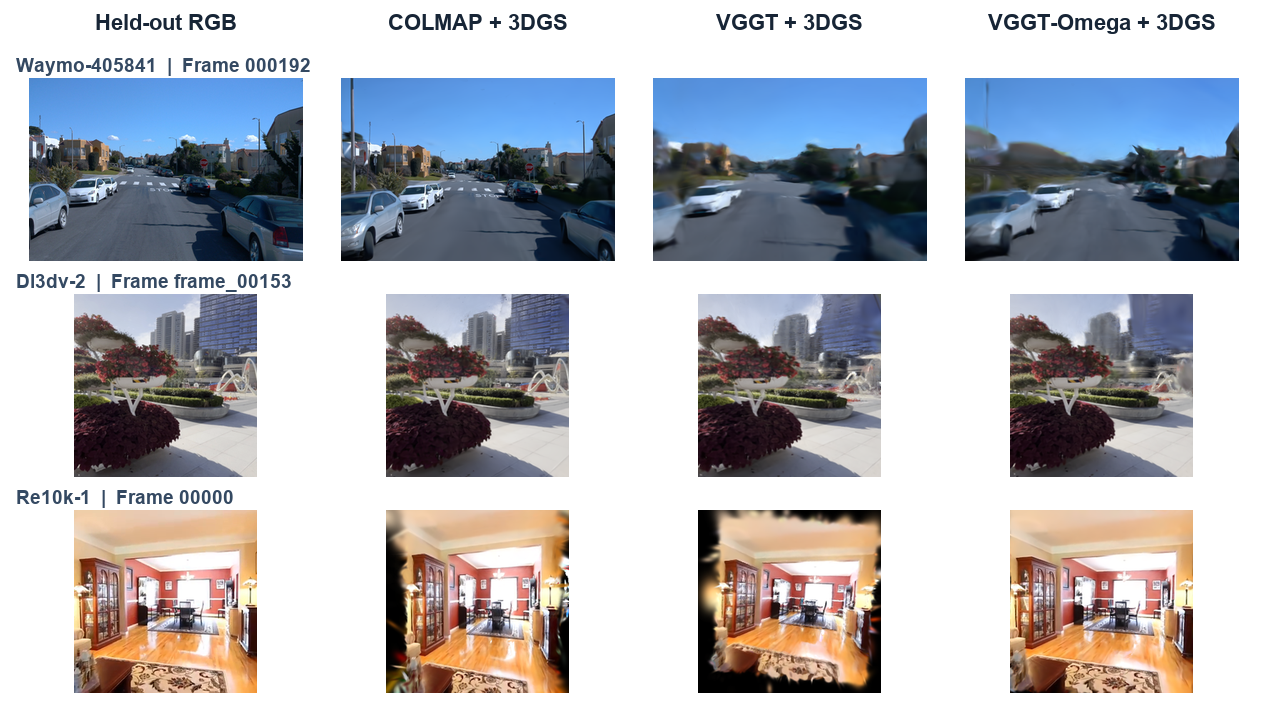
\includegraphics[width=0.94\textwidth]{part1_comparison.png}
  \caption{Example held-out images and the corresponding raw 3DGS renders from the three candidate initializers. Each row uses the same target camera across methods.}
  \label{fig:dense_qual}
\end{figure*}

\begin{figure*}[!t]
  \centering
  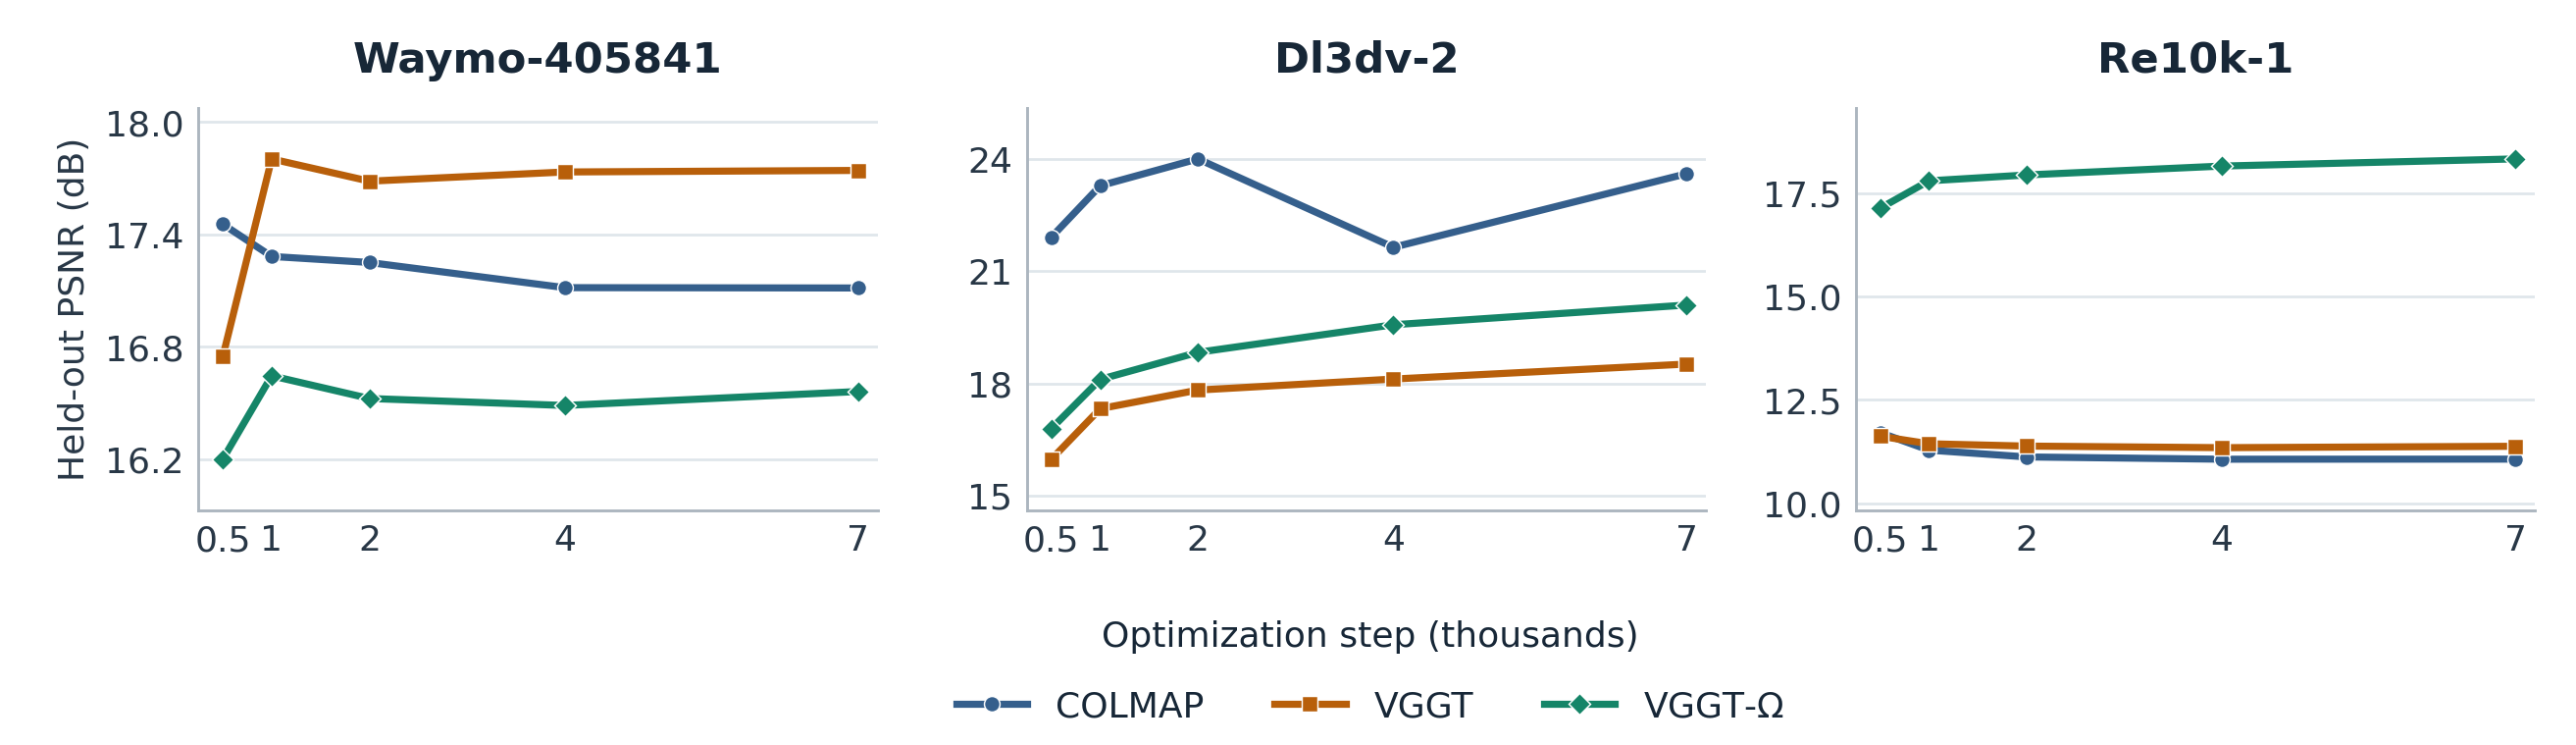
\includegraphics[width=0.94\textwidth]{convergence.png}
  \caption{Dense-view PSNR over the same five checkpoint steps. Several conditions reach their best measured test PSNR before the fixed endpoint.}
  \label{fig:dense_convergence}
\end{figure*}

\paragraph{Initialization cost.}
VGGT-$\Omega$ initializes in 36--42~s and has the shortest end-to-end runtime on all three sequences (Table~\ref{tab:dense}). It is 2.1--2.9$\times$ faster to initialize than VGGT and 9.7--22.3$\times$ faster than our COLMAP configuration. For context, COLMAP uses 8 CPU workers for Waymo and RealEstate10K and 4 for DL3DV. The Waymo matcher uses a 200-image block for 174 input frames to avoid a repeated multi-block failure, and the other scenes use blocks of 50. Earlier camera settings registered only 107 of 174 Waymo views and 66 of 244 RealEstate10K views. Every final COLMAP run registers all training frames. These timing comparisons describe complete working configurations, including their different neural resolutions and SfM settings.

\paragraph{Reconstruction quality.}
On DL3DV, COLMAP leads all quality metrics and has a 3.51~dB PSNR margin over the next best method. Its renders preserve foreground contours and the fa\c{c}ade more clearly (Fig.~\ref{fig:dense_qual}). On RealEstate10K, VGGT-$\Omega$ improves PSNR by 6.95~dB over VGGT and better preserves furniture contours and image borders. On Waymo, VGGT reaches the highest PSNR and SSIM, while COLMAP has better LPIPS and smaller center error. One aligned trajectory score therefore explains only part of the quality ranking.

\paragraph{Convergence and resource use.}
DL3DV's neural initializers improve through all reported checkpoints. COLMAP peaks at 24.00~dB at step 2,000, dips to 21.64~dB at 4,000, then recovers to 23.61~dB (Fig.~\ref{fig:dense_convergence}). RealEstate10K's VGGT-$\Omega$ gains 1.19~dB between steps 500 and 7,000. The nine trained scenes yield 389,467 to 721,872 Gaussians and peak allocated training memory of 0.66--1.30~GiB. Differences in initialization cost are larger than training-time differences within each scene.

\subsection{Part 2: Full versus sparse unposed input}
\label{sec:part2}

\begin{table*}[!t]
  \centering\small
  \begin{tabular}{llrrrrrrr}
    \toprule
    Scene & Input & PSNR (dB) $\uparrow$ & SSIM $\uparrow$ & LPIPS $\downarrow$ & Paired ATE $\downarrow$ & Init. (s) & Train (s) & Total (s) \\
    \midrule
    Waymo & Full & \textbf{17.689} & \textbf{0.6542} & 0.5204 & 0.95649 & 661.5 & 563.8 & 1322.4 \\
          & Sparse & 16.726 & 0.5971 & \textbf{0.4574} & \textbf{0.72937} & 109.0 & 703.7 & 901.2 \\
    DL3DV & Full & \textbf{18.609} & \textbf{0.5142} & \textbf{0.1843} & 0.03790 & 836.5 & 308.1 & 1198.5 \\
          & Sparse & 15.479 & 0.4559 & 0.2572 & \textbf{0.02903} & 79.3 & 160.0 & 273.7 \\
    RealEstate10K & Full & \textbf{11.364} & \textbf{0.2910} & \textbf{0.3957} & 0.02902 & 925.9 & 474.8 & 1459.4 \\
                  & Sparse & 11.234 & 0.2751 & 0.4055 & \textbf{0.02643} & 69.3 & 321.9 & 427.3 \\
    \bottomrule
  \end{tabular}
  \caption{Part 2 at 7,000 steps. Paired ATE evaluates both models on the same sparse training camera IDs. Initialization and training columns are the internal stage timers. Total sums initialization, training, rendering, and evaluation subprocess wall-clock times, including their startup and I/O.}
  \label{tab:sparse}
\end{table*}

\begin{figure*}[!t]
  \centering
  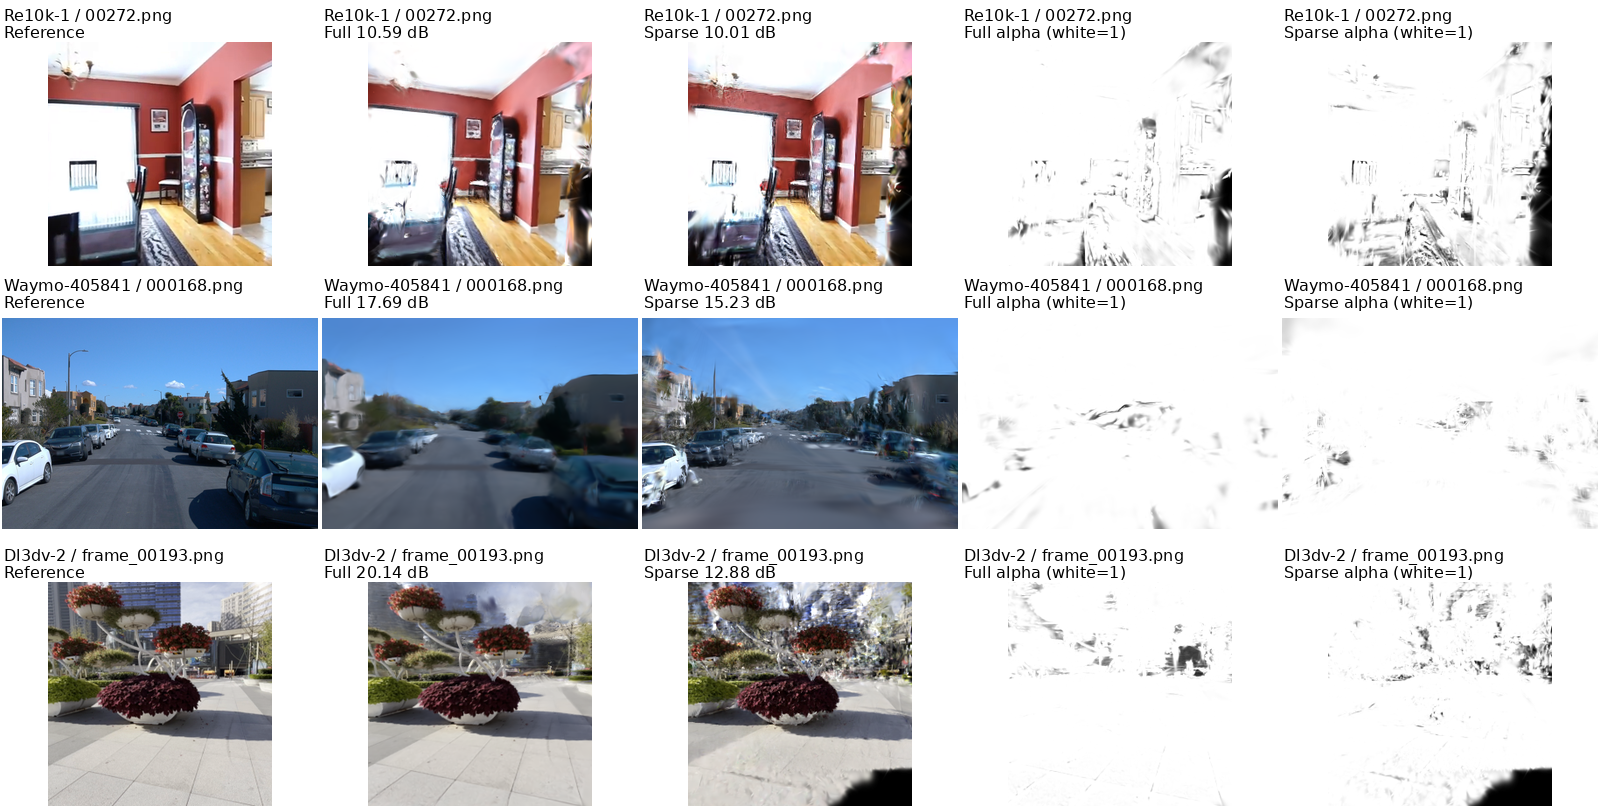
\includegraphics[width=0.94\textwidth]{failure_cases.png}
  \caption{Within each scene, the held-out view with the largest full-minus-sparse PSNR gap. The last two columns show accumulated alpha as projected support (white is opaque). The view selection illustrates failure modes, and the quantitative comparison evaluates every held-out view.}
  \label{fig:sparse_failures}
\end{figure*}

\ifpartthreeevidence\partthreeassets\fi

\paragraph{Rendering and runtime.}
Full input improves average PSNR and SSIM on all three sequences. The largest PSNR change is 3.13~dB on DL3DV. Waymo shows a metric split: full achieves higher PSNR on 24 of 25 views, while sparse achieves lower LPIPS on all 25 views. With fewer cameras, initialization falls from 661--926~s to 69--109~s. The sparse Waymo model takes longer to optimize and finishes with about 839,000 Gaussians, compared with 484,000 in the full condition. The sparse total time is nevertheless lower in each scene (Table~\ref{tab:sparse}).

\paragraph{Pose and visibility.}
Sparse has lower center ATE on the shared camera IDs, but on Waymo its mean orientation discrepancy increases from $1.05^\circ$ to $2.21^\circ$. Re10k's independent full and sparse VGGT initializations both estimate focal lengths approximately 20\% above the supplied reference. Figure~\ref{fig:sparse_failures} shows a cabinet boundary distorted in both Re10k conditions and fragmented foliage and dark ground regions in sparse DL3DV. The mean fraction of test pixels with alpha at least 0.9 falls from 95.98\% to 92.29\% in DL3DV and from 87.27\% to 83.69\% in Re10k. Alpha measures projected support. Incorrect opaque structures can still have high accumulated alpha.

\paragraph{Convergence and replay.}
Sparse Re10k and Waymo peak early in the observed checkpoints, while sparse DL3DV's highest sampled PSNR exceeds the last checkpoint by 0.63~dB. The \href{https://github.com/MoliaiELS/CV_Project4/blob/main/results/part2_supplement_v1/figures/convergence_all_metrics.png}{archived curves} retain all five measurements per metric. Replay of all three archived Part 1 VGGT checkpoints on the course GPU reproduces their archived final PSNR at six decimal places. Those full results are within 0.09~dB of the independently trained Part 2 full runs. The primary contrast uses the native Part 2 pairs.

\subsection{Part 3: Generative reconstruction}
\label{sec:part3}
\ifpartthreeevidence
\partthreeresults
\else
The evaluation compares the initial sparse checkpoint $M_0$ and the Gaussian scenes from every round with a real-only continuation at the same step. Raw held-out renders use the fixed Part 2 test cameras. The restored virtual views and confidence maps describe where the method applies new supervision; the held-out comparison tests whether the updates generalize.

\emph{Part 3 evidence to be loaded from verified run artifacts before submission.}
\fi


\section{Discussion and conclusion}
Feed-forward geometry shortens dense initialization, with scene-dependent quality gains. Camera orientation, intrinsics, and visibility also affect sparse rendering quality. Generative feedback adds supervision between real views and can propagate inconsistent edits.

\ifpartthreeevidence\partthreeconclusion\fi

The small scene set and one seed per condition limit generalization. DL3DV data were used to train Difix and DA3~\cite{wu2025difix,lin2025da3}. Exact overlap between course scenes and pretrained model corpora is unknown. The project split reserves held-out images for evaluation. Fixed cameras and Gaussian topology limit geometric recovery, and opaque errors can still score high on alpha. Future tests could measure geometry on Tanks and Temples~\cite{knapitsch2017tanks} and assess temporally coherent completion with video diffusion caches~\cite{liu2025teacache,haghighi2026sencache}.

% Reset the two-column page after flushing wide figures.
\onecolumn
\twocolumn
{\small
\setlength{\bibsep}{0pt}
\bibliographystyle{ieeenat_fullname}
\bibliography{part1_refs,final_refs}
}
\end{document}
